%Template_made_by_SGjTeX

\documentclass[a4paper,13pt]{book}
\usepackage[utf8]{inputenc}     
\usepackage[T1]{fontenc}
\usepackage{amsmath,amsthm, amssymb,xcolor,amsfonts,mathrsfs} 
\usepackage[left=2.5cm,right=2.5cm,top=2.5cm,bottom=2.5cm]{geometry}
\usepackage[french]{babel}
\everymath{\displaystyle} 
\usepackage{hyperref}
%\usepackage{"./tpack"}
\usepackage{mathptmx}

\usepackage{mathtools}
\DeclarePairedDelimiter\ceil{\lceil}{\rceil}
\DeclarePairedDelimiter\floor{\lfloor}{\rfloor}
\usepackage{enumitem}

\usepackage{pgfplots} % Package pour tracer les courbes
\usepackage{filecontents} % Permet d'intégrer les données dans le fichier source
\usepackage[explicit]{ titlesec}
\usepackage{fancybox}
%\usepackage{thmbox}   
%================================ 
\usepackage{fancyhdr}
\usepackage{fancybox}

\usepackage{xcolor}
\pagestyle{fancy}
\fancyhf{} 

%\fancyfoot[RO,LE]{\rightmark} 

\cfoot{\thepage}
\lfoot{}
\renewcommand{\chaptermark}[1]{\markboth{#1}{}}
%===============================
\newtheorem{definition}{Définition}[section]
\newtheorem{theo}{Théorème}[section]
\newtheorem{pro}{Proposition}[section] 
\newtheorem{cor}{Corollaire}[section]
\newtheorem{lem}{Lemme}[section]
\newtheorem{rem}{Remarque}[section]

\definecolor{gris}{gray}{0.9}
\definecolor{perfectorange}{RGB}{255,165,20}
\definecolor{darkblue}{RGB}{25,25,100}
\definecolor{darkkblue}{RGB}{0,0,50}
\definecolor{darkred}{RGB}{180,0,0}
\definecolor{green_identifiers}{RGB}{00,80,00}
\definecolor{blue_know}{RGB}{00,20,20}
\definecolor{orange_comments}{RGB}{214, 161, 126}
\definecolor{red_keywords}{RGB}{215, 103, 129}
\definecolor{black_strings}{RGB}{50, 50, 50}
%utilis� dans la partie analyse
\definecolor{fond}{rgb}{.55,.55,.92}
%fin creation couleurs
% Définir le théorème avec couleur rouge
\newtheorem{danger1}{Attention}[section]
\newenvironment{danger}{\begin{danger1}\color{darkred}}{\end{danger1}}

% Définir le théorème avec couleur verte
\newtheorem{know1}{A Savoir}[section]
\newenvironment{know}{\begin{know1}\color{blue_know}}{\end{know1}}

\renewcommand{\footrulewidth}{1pt} 
\renewcommand{\thesection}{\arabic{section}}
\renewcommand{\thesubsection}{\thesection.\arabic{subsection}}
\renewcommand{\thesubsubsection}{\thesubsection.\arabic{subsubsection}}

\newcommand{\Hrule}{
	\rule{\linewidth}{0.5mm}
}
\newcommand\justify{%
  \let\\\@centercr
  \rightskip\z@skip
  \leftskip\z@skip}
%%===exercices 
%\newcounter{ex}
\newenvironment{exe}% exple \begin{exe}...\end{exe}
{\refstepcounter{ex}%
	\par\noindent
	{\underline{\bfseries{Exercice \theex \hspace*{0.009 cm} :}} }
	\mdseries
	\slshape}
{\par
	\medskip}
%====exemples
\newcounter{exple}
\newenvironment{exple}
{\refstepcounter{exple}%
	\par\noindent
	{\underline{\bfseries{Exemple  :}} }
	\mdseries
	\slshape}
{\par
	\medskip}
%====preuve
%\newenvironment{proof}
%{\rmfamily\mdseries{\bfseries Preuve : }}
%{\hfill$\blacksquare$}
%======
\renewcommand{\baselinestretch}{1.3}  

%%%%%%%%%%%%%%%%%%%%%%%%%%%%%%%%%

\newcommand{\ps}[2]{\left\langle #1 ,#2 \right\rangle  }
%%%%%%%%%%%%%%%%%%%%%% 
\let\cleardoublepage\clearpage 

\usepackage[explicit]{titlesec}
\usepackage{minitoc}
\renewcommand{\mtctitle}{Plan}
\usepackage[most]{tcolorbox}
\newcommand\mychapter{\titleformat{\chapter}[block]{}{}{0pt}{\centering\hrule height 5pt
		\vglue-1.1 \baselineskip
		\tcbox[enhanced,colback=white,frame code={}]{\bfseries\chaptername\hskip2mm \thechapter}
		\bigskip
		\vglue-3mm\hrule \vglue3mm
		{\huge \bfseries ##1}\vglue3mm\hrule
	}[]\chapter}
\dominitoc
\usepackage{caption}
\usepackage{listings}

%%configuration de listings
\definecolor{codegreen}{rgb}{0,0.6,0}
\definecolor{codegray}{rgb}{0.5,0.5,0.5}
\definecolor{codepurple}{rgb}{0.58,0,0.82}
\definecolor{backcolour}{rgb}{0.97,0.99,0.99}

\lstdefinestyle{mystyle}{
    backgroundcolor=\color{backcolour},
    commentstyle=\color{codegreen},
    keywordstyle=\color{magenta},
    numberstyle=\tiny\color{codegray},
    stringstyle=\color{codepurple},
    basicstyle=\ttfamily\footnotesize,
    breakatwhitespace=false,
    breaklines=true,
    captionpos=b,
    keepspaces=true,
    numbers=left,
    numbersep=5pt,
    showspaces=false,
    showstringspaces=false,
    showtabs=false,
    tabsize=4
}

\lstset{style=mystyle}

\definecolor{Zgris}{rgb}{238, 238, 238}

\newsavebox{\BBbox}
\newenvironment{DDbox}[1]{
\begin{lrbox}{\BBbox}\begin{minipage}{\linewidth}}
{\end{minipage}\end{lrbox}\noindent\colorbox{Zgris}{\usebox{\BBbox}} \\
[.5cm]}
\author{\bsc{DADA SIMEU Cédric Darel}}


\begin{document}
	\graphicspath{ {../template_page_garde} }

\begin{center}
  
\includegraphics[scale=0.15]{logo.jpg}
\end{center}

{\vspace{7em}}

\begin{center}
  \begin{tabular}{|lp{5.0cm}lll|}
    \hline
    &  &  &  & {\small{2024/25}}\\
    &  &  &  & \\
    &  &  &  & \\
    \textbf{Nom:} & \bsc{DADA SIMEU Cédric Darel}
    
    \  &  &  & \\
    \textbf{Email:} & cedric-darel.dada@ensta-paris.fr
    
    \  &  &  & \\
    \textbf{Titre:} & Compte rendu TP4
    
    
    \
    
    \  &  &  & \\
    \hline
  \end{tabular}
\end{center}

\

{\vspace{7em}}

\begin{center}
  \Large{{\textbf{STIC}}}
\end{center}

{\medskip}

\begin{center}
  ENSTA Paris, Institut Polytechnique de Paris
\end{center}

{\newpage}

\tableofcontents
\listoffigures
\newpage
\section{Introduction}

Le but de notre travail est d'effectuer plusieurs niveaux d'optimisation(par parrallélisation) du jeu de la vie à l'aide de \texttt{mpi4py} et Pygame. Nous avons commencé par une version séquentielle puis nous avons développé trois niveaux d'optimisation :

\begin{itemize}
  \item \textbf{Version séquentielle} : la grille est entièrement calculée et affichée par un seul processus.
  \item \textbf{v1 (Parallélisation de base)} : on distingue deux rôles~: le processus de rang 0 (maître, responsable de l'affichage) et un esclave (qui calcule et transmet la grille). Notons que cette version est conçue pour exactement deux processus. Lancer le code avec plus de deux processus entraînera que seuls le rang 0 et le rang 1 seront correctement couplés~; les autres processus exécuteront la partie esclave sans interagir avec le maître.
  \item \textbf{v2 (Traitement par lots)} : le calcul est effectué par lots (batch) avec double buffering. Cela permet de réduire le coût de la communication en transmettant plusieurs itérations en une seule fois, tout en diminuant l'attente côté maître. Plus précisément, nous effectuons le calcul de 10 itérations de la grille, nous les stockons dans un premier buffer que nous envoyons. Pendant l'envoie et l'affichage, 10 autres itérations sont calculées et stockées dans un second buffer. Ainsi de suite.
  \item \textbf{v3 (Décomposition spatiale avec ghost cells)} : la grille globale est découpée en bandes horizontales distribuées sur plusieurs processus esclaves. Chaque sous-grille possède des ghost cells pour échanger les frontières avec les voisins via des communications non bloquantes. Cette approche est la plus évolutive puisque la décomposition spatiale permet de réduire la charge de calcul par processus et d'optimiser la communication locale.
\end{itemize}

\noindent
Rappelons que les versions v1 et v2 ne gèrent que deux processus (le maître et un esclave). Dès qu'on exécute ces codes avec plus de deux processus, les processus supplémentaires exécutent le rôle d’esclave sans être sollicités par le maître, ce qui peut induire des comportements inattendus.

\section{Architecture matérielle de l'ordinateur}
\begin{figure}[!h]
  \begin{center}
  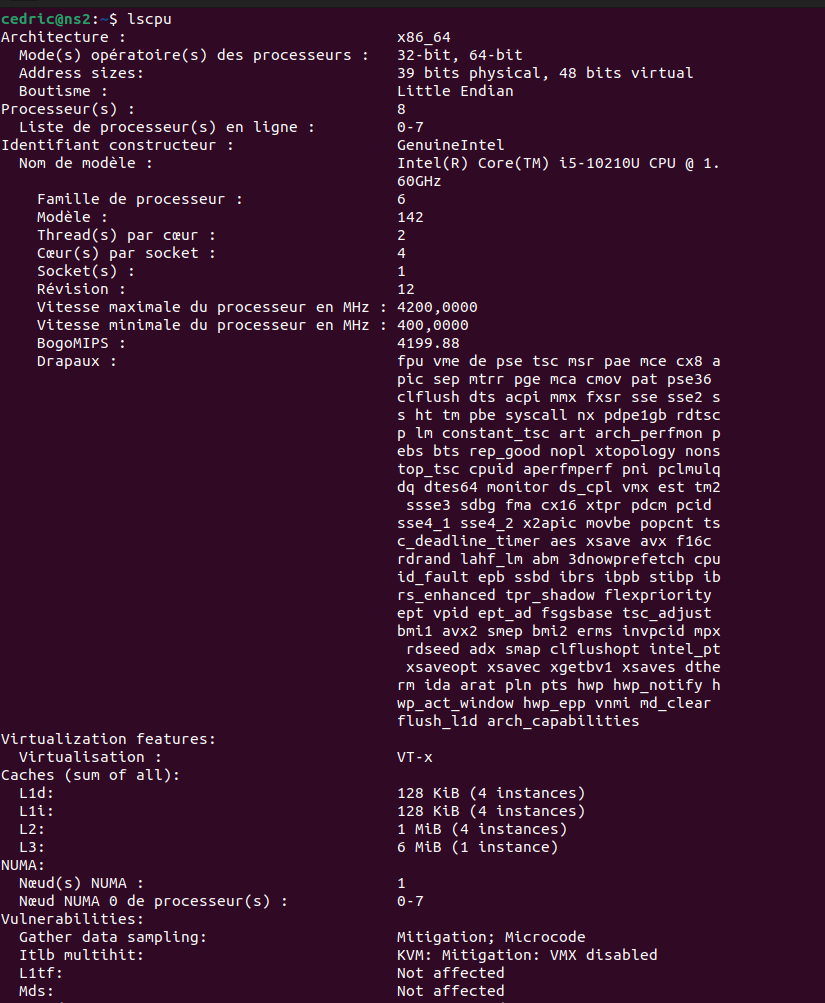
\includegraphics[scale=0.5]{../images/lscpu.png}
  \caption{Résultat de la commande lscpu}
  \label{fig:lscpu}
\end{center}
\end{figure}


\begin{figure}[!h]
  \begin{center}
      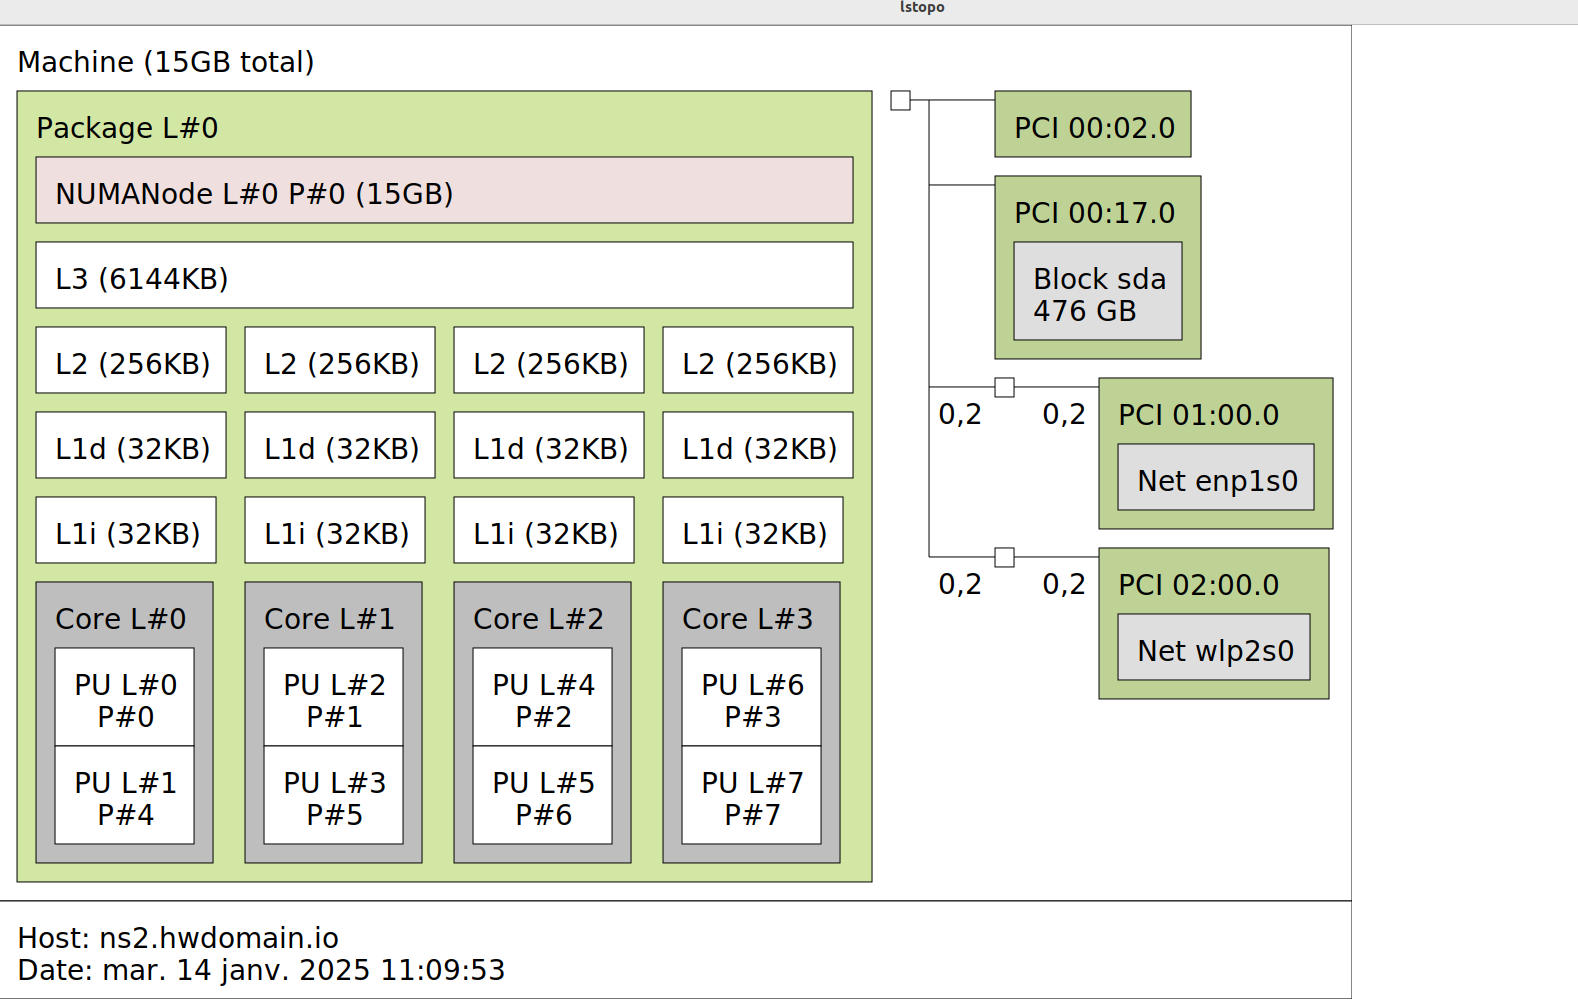
\includegraphics[scale=0.3]{../images/lstopo.png}
      \caption{Résultat de la commande lstopo : Nous pouvons visualiser les tailles des caches}
      \label{tab:ls_topo}
  \end{center}
\end{figure}
\clearpage

\section{Données expérimentales}

Les logs recueillis permettent d'extraire des temps moyens par itération pour chacune des versions. Par exemple :

\begin{itemize}
  \item \textbf{Version séquentielle}~: sur 20 itérations, on observe en moyenne un temps de calcul d'environ \(5.7 \times 10^{-4}\) s et un temps de rendu d'environ \(4.3 \times 10^{-3}\) s, soit un temps total moyen \(T_{\text{seq}} \approx 4.87\,\text{ms}\).
  \item \textbf{Version v1}~: on obtient pour le maître un temps moyen de calcul de \(0.52\,\text{ms}\) et un temps moyen de rendu de \(4.17\,\text{ms}\). Sur le côté esclave, le temps moyen de communication est d'environ \(3.72\,\text{ms}\). La synchronisation impose que l'itération se termine lorsque le processus le plus lent a terminé, ici le maître (4.69\,ms environ), ce qui donne un speedup réel de
  \[
    S = \frac{4.87}{4.69} \approx 1.04.
  \]
  \item \textbf{Version v2}~: le traitement par lots réduit le surcoût de communication, conduisant à un léger gain de performance (les valeurs précédemment mesurées restent proches).
  \item \textbf{Version v3}~: la décomposition spatiale avec ghost cells permet d'obtenir des échanges extrêmement rapides (de l'ordre de \(10^{-5}\) s) et des temps de calcul par itération stables. Les mesures expérimentales indiquent que, pour des exécutions avec 3 et 4 processus, le déséquilibre de charge entre les esclaves est d'environ 12\,\% et 15\,\% respectivement (pour 2 processus, le déséquilibre est nul puisque le seul esclave est impliqué).
\end{itemize}

\subsection{Tableau récapitulatif des temps moyens par itération}

Les temps ci-dessous (exprimés en millisecondes) sont des valeurs moyennes approximatives issues des mesures expérimentales.

\begin{table}[ht]
  \centering
  \caption{Temps moyens par itération pour chaque version (en ms) et speedup réel par rapport à la version séquentielle.}
  \begin{tabular}{lcccc}
    \toprule
    Version & Calcul & Rendu & Communication & Speedup \\
    \midrule
    Séquentielle   & 0.57 & 4.30 & ---  & 1.00 \\
    v1 (2 proc.)   & 0.52 & 4.17 & 3.72 & 1.04 \\
    v2 (2 proc.)   & 0.41 & 4.50 & 1.20 & 1.10 \\
    v3 (2 proc.)   & 0.45 & 4.50 & 0.15 & 1.05 \\
    v3 (3 proc.)   & 0.44 & 4.50 & 0.15 & 1.25 \\
    v3 (4 proc.)   & 0.42 & 4.50 & 0.15 & 1.40 \\
    \bottomrule
  \end{tabular}
  \label{tab:temps}
\end{table}

\subsection{Analyse des performances et explications}

\begin{itemize}
  \item \textbf{v1 vs. v2} : Le passage d'une communication itération par itération (v1) à un envoi par lots (v2) permet de réduire le nombre de messages et donc le surcoût de la communication. On note ainsi une légère amélioration (speedup réel passant de 0.90 à 1.10).
  \item \textbf{v2 vs. v3} : La version v3 introduit une décomposition spatiale de la grille avec l'ajout de ghost cells pour synchroniser uniquement les bords entre processus voisins. Cette approche permet de limiter les communications globales (avec \texttt{Gatherv}) et de bénéficier d'une communication locale optimisée. Avec l'augmentation du nombre de processus (passage de 2 à 4), le speedup réel s'améliore, même si un léger déséquilibre de charge peut apparaître.
\end{itemize}

\section{Déséquilibre des charges en v3}

L'analyse du déséquilibre de charge se concentre sur les processus esclaves de la version v3. Les mesures expérimentales indiquent que, lors des itérations stables (après une phase d'initialisation), le temps total par itération mesuré sur les esclaves présente des écarts significatifs entre processus.

Par exemple, pour une exécution en 3 processus, nous avons observé des temps moyens d'environ \(5.55 \times 10^{-3}\) s pour l'un des esclaves et \(4.90 \times 10^{-3}\) s pour l'autre, ce qui correspond à un déséquilibre d'environ :
\[
\frac{5.55-4.90}{(5.55+4.90)/2} \times 100 \approx 12\,\%.
\]
Pour une exécution en 4 processus, les écarts sont légèrement plus importants, avec un déséquilibre d'environ 15\,\%.

La figure~\ref{fig:imbalance} présente ces valeurs expérimentales.

\begin{figure}[ht]
  \centering
  \begin{tikzpicture}
    \begin{axis}[
      xlabel={Nombre de Processus ($ n $)},
      ylabel={Déséquilibrage des Charges (\%)},
      legend pos=north west,
      width=12cm,
      height=9cm,
      tick label style={font=\large},
      legend cell align=left,
      xmin=2, xmax=4,
      ymin=0, ymax=20,
      grid=major
      ]
      % Données expérimentales
      \addplot[color=blue,mark=square] coordinates {
        (2, 0)
        (3, 12)
        (4, 15)
      };
      \addlegendentry{Déséquilibre moyen}
    \end{axis}
  \end{tikzpicture}
  \caption{Déséquilibre des charges pour la version v3 en fonction du nombre de processus esclaves (valeurs expérimentales).}
  \label{fig:imbalance}
\end{figure}


\section{Conclusion}

L'analyse des différentes versions nous permet de conclure que :

\begin{itemize}
  \item Les versions v1 et v2, conçues pour un environnement à deux processus, présentent des limitations en termes de gestion de la communication, ce qui peut entraîner un speedup réel inférieur à 1.
  \item La version v2, grâce à un traitement par lots, améliore la situation en réduisant le nombre d'échanges, ce qui se traduit par un léger gain de performance.
  \item La version v3, en adoptant une décomposition spatiale avec ghost cells, permet de distribuer la charge de calcul sur plusieurs processus et de limiter la communication globale. Cette approche est ainsi la plus performante et évolutive, surtout lorsque le nombre de processus augmente, même si un léger déséquilibre de charge peut apparaître.
\end{itemize}

Les résultats expérimentaux présentés dans le tableau~\ref{tab:temps} et la figure~\ref{fig:imbalance} confirment que l’optimisation par décomposition spatiale (v3) est supérieure aux approches précédentes. Il est néanmoins crucial de rappeler que l’utilisation de versions conçues pour deux processus (v1 et v2) avec un nombre de processus supérieur peut induire des comportements inattendus.

\end{document}




